\chapter{METODOLOGI}
\label{chap:metodologi}

\section{Metode yang digunakan}
\label{sec:metode}

Penelitian ini dilaksanakan sesuai dengan metodologi yang telah dirancang. 
Metodologi terbagi menjadi 4 tahap, yaitu pengumpulan data, pembentukan arsitektur GAN, training model, dan evaluasi model. 
Gambar \ref{fig:metodologi} menunjukkan diagram dari metodologi penelitian.

\begin{figure}[ht]
  \centering
  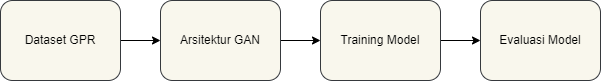
\includegraphics[scale=0.7]{gambar/metodologi.png}
  \caption{Diagram Metodologi Penelitian}
  \label{fig:metodologi}
\end{figure}

\subsection{Dataset GPR}
\label{subsec:datasetgpr}

Tahap ini merupakan tahap pengumpulan dataset GPR. 
Data yang dibutuhkan ada 2 jenis, yaitu data input berupa gambar B-scan GPR hasil simulasi gprMax dan data output yang diharapkan berupa gambar bentuk geometri dari gambar B-scan GPR. 
Alur dari proses pengumpulan dataset ditampilkan pada gambar \ref{fig:datasetgpr}.

\begin{figure}[ht]
  \centering
  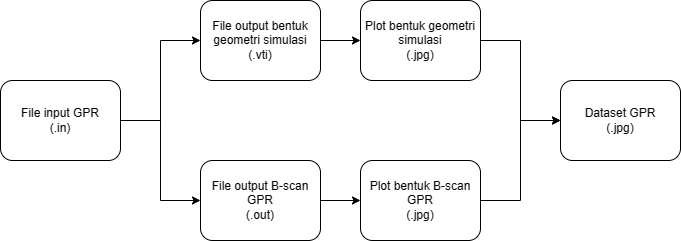
\includegraphics[scale=0.7]{gambar/alur pengumpulan data.png}
  \caption{Diagram Pengumpulan Dataset GPR}
  \label{fig:datasetgpr}
\end{figure}

Simulasi menggunakan gprMax untuk menghasilkan file output bentuk geometri simulasi dan file output B-scan GPR dengan menggunakan file input gprMax. 
Setiap kebutuhan dan cara instalasi gprMax dapat diperoleh di github gprMax. 
Dalam memasang gprMax, dibutuhkan untuk memasang Python, Miniconda/Anaconda, dan C Compiler yang mendukung OpenMP (Desktop development with C++ pada Visual Studio untuk OS Windows). \\

Dalam menyusun kode program input GPR, dibutuhkan beberapa parameter penyusun yang perlu diperhatikan. 
Parameter penyusun tersebut dapat dilihat pada panduan gprMax di website resmi gprMax. 
Pada penelitian ini, parameter sistem yang dibuat pada dataset GPR dapat dilihat pada tabel \ref{tb:inputGPR}. 
Contoh penggunaan parameter pada file input juga dapat dilihat pada gambar \ref{fig:inputgprMax}.

\begin{longtable}{|c|c|c|}
  \caption{Parameter Input GprMax}
  \label{tb:inputGPR}                                   \\
  \hline
  \rowcolor[HTML]{C0C0C0}
  \textbf{Parameter} & \textbf{Nilai} \\
  \hline
  Dimensi                     & 0.3 m x 0.3 m x 0.001 m                   \\
  Jendela Waktu               & 3 ns                                      \\
  Material                    & Beton (medium) dan ruang kosong (objek)   \\
  Basis Sinyal                & Ricker                                    \\
  Arah Laju Sumber Sinyal     & 0.001 m/step terhadap sumbu-X             \\
  Bentuk Objek                & Tabung                                    \\
  \hline
\end{longtable}

\begin{figure}[ht]
  \centering
  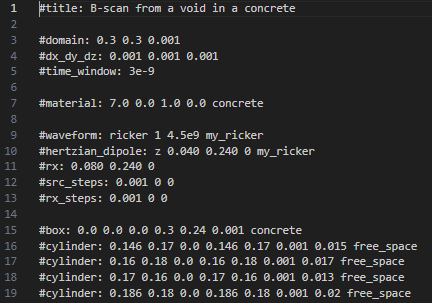
\includegraphics[scale=1]{gambar/inputGprMax.png}
  \caption{Contoh isi file input gprMax}
  \label{fig:inputgprMax}
\end{figure}

Data input gprMax di atas kemudian disimulasikan dengan 2 tools berbeda untuk menghasilkan file output bentuk geometri simulasi dan file output B-scan GPR. 
Dari proses simulasi, diperoleh dua buah hasil, yaitu file output bentuk geometri simulasi (.vti) dan file output B-scan GPR (.out). 
Untuk memperoleh gambar bentuk geometri simulasi, file output bentuk geometri simulasi dijalankan menggunakan aplikasi Paraview. 
Sedangkan untuk memperoleh gambar bentuk sinyal B-scan GPR, file output B-scan GPR dijalankan menggunakan tools dari gprMax.

Kedua jenis gambar ini kemudian digabung menjadi satu gambar dengan menggunakan library PIL. 
Kedua gambar akan disusun horizontal, dimana gambar yang kiri berupa gambar B-scan gprMax dan gambar yang kanan berupa gambar bentuk geometrinya. 
Contoh gabungan gambar ditampilkan pada gambar \ref{fig:contohdata}. 
Gambar hasil gabungan ini yang kemudian menjadi dataset model GAN yang akan dibentuk, yang dalam penelitian ini menggunakan sejumlah 200 data.

\begin{figure}[ht]
  \centering
  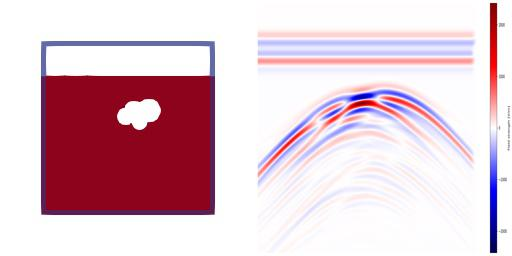
\includegraphics[scale=0.7]{gambar/data1.jpg}
  \caption{Gambar gabungan bentuk geometri bawah permukaan (kiri) dengan bentuk B-scan GPR hasil simulasi (kanan)}
  \label{fig:contohdata}
\end{figure}

\subsection{Arsitektur GAN}
\label{subsec:arsitekturGAN}

Setelah dataset berhasil dikumpulkan, selanjutnya akan dibentuk model dari GAN. 
Model GAN yang akan dibentuk menggunakan model Conditional GAN Pix2pix. 
Arsitektur GAN akan dibagi menjadi 2 bagian, yaitu bagian generator yang berfungsi untuk mensintesis gambar seperti data asli, dan bagian diskriminator yang berfungsi untuk membedakan antara data asli dengan data hasil sintesis. 
Bentuk arsitektur GAN ditampilkan pada gambar \ref{fig:arsitekturGAN}.

\begin{figure}[ht]
  \centering
  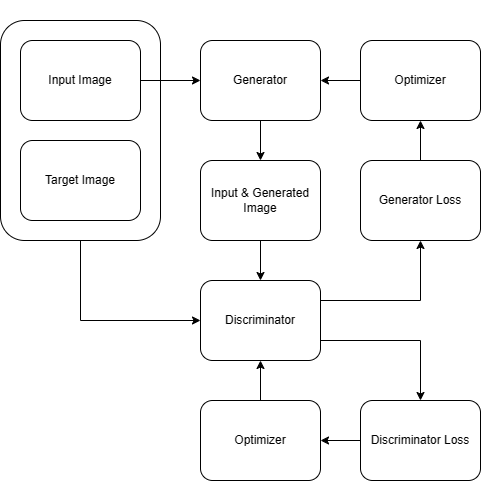
\includegraphics[scale=0.5555]{gambar/Arsitektur GAN.png}
  \caption{Diagram Arsitektur GAN yang Dibentuk}
  \label{fig:arsitekturGAN}
\end{figure}

\newpage

Pada bagian generator, digunakan arsitektur U-net \parencite{UNet}. 
Arsitektur ini terdiri dari jaringan encoder yang dilanjut dengan jaringan decoder. 
Jaringan encoder akan menerapkan proses Convolution $>>$ Batch normalization $>>$ Leaky ReLU. 
Sedangkan decoder akan menerapkan proses Transposed convolution $>>$ Batch normalization $>>$ Dropout (untuk 3 blok pertama) $>>$ ReLU. 
Tiap pasang encoder-decoder memiliki skip connection yang berfungsi untuk menangkap setiap informasi tingkat rendah yang dibagikan antara input dan output. 
Diagram arsitektur Generator dapat dilihat pada gambar \ref{fig:generator}.

\begin{figure}[ht]
  \centering
  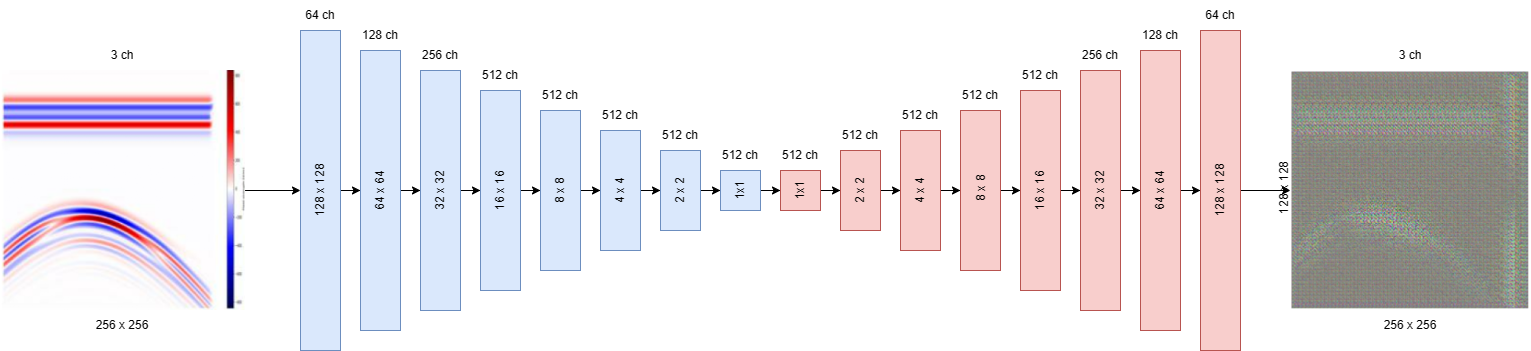
\includegraphics[scale=0.25]{gambar/Generator.png}
  \caption{Diagram Arsitektur Generator}
  \label{fig:generator}
\end{figure}

Pada bagian discriminator, digunakan arsitektur Convolutional Patch GAN yang akan mencoba mengklasifikasikan sepetak (30 x 30) gambar itu nyata atau tidak. 
Discriminator akan menerima dua pasang gambar sebagai input, yaitu gambar input-asli dan gambar input-sintesis. 
Masing-masing pasangan input ini akan digabung terlebih dahulu sebelum masuk ke jaringan encoder. 
Diagram arsitektur Discriminator dapat dilihat pada gambar \ref{fig:discriminator}.

\begin{figure}[ht]
  \centering
  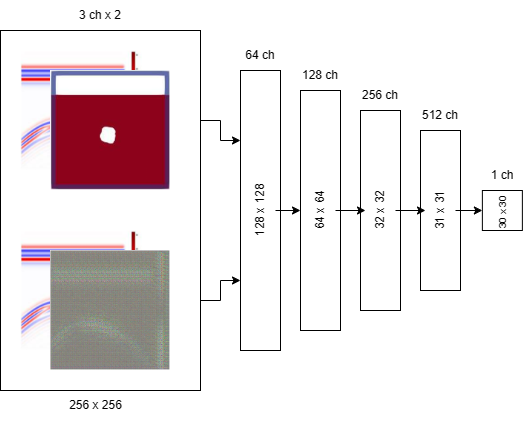
\includegraphics[scale=0.5]{gambar/Discriminator.png}
  \caption{Diagram Arsitektur Discriminator}
  \label{fig:discriminator}
\end{figure}

Generator Loss merupakan gabungan dari sigmoid cross-entropy loss antara gambar yang dihasilkan dengan suatu array 1 (GAN Adversial Loss), dan MAE (Mean Absolute Error) antara gambar yang disintesis dengan gambar asli(L1 Loss). 
Secara matematis, nilai dari Total Generator Loss dapat didefinisikan sebagai 

\begin{equation}
  \label{eq:genLoss}
  Total Generator Loss = GAN Adversial Loss + (Lambda * L1 Loss) 
\end{equation}

dimana Lambda dapat didefisinikan sesuai keinginan model (pada penelitian ini Lambda = 100).

Discriminator Loss terdiri dari sigmoid cross-entropy loss antara gambar asli dengan array 1 (Real Loss), dan sigmoid cross-entropy loss antara gambar yang dihasilkan dengan array 0 (Generated Loss). 
Total Discriminator Loss merupakan jumlah dari Real Loss dan Generated Loss

Pada model GAN juga didefinisikan fungsi optimizer dan checkpoint.
Fungsi optimizer menggunakan Adaptive Moment Estimation (Adam) baik untuk generator maupun diskriminator. 
Fungsi checkpoint digunakan untuk menyimpan hasil sementara (checkpoint) dari hasil pelatihan generator dan diskriminator model GAN.

\subsection{Training Model}
\label{training}

Arsitektur GAN yang telah dibentuk kemudian diteruskan ke proses training. 
Alur keseluruhan Training Model dapat dilihat pada gambar \ref{fig:training}. 
Dari 200 data pada dataset, 160 digunakan untuk proses training model. 
Proses training model ini dilakukan sebanyak 40000 iterasi. 
Untuk setiap 1000 iterasi, akan ditampilkan proses sintesis gambar, dan untuk setiap 5000 iterasi, checkpoint dari model akan disimpan.

\begin{figure}[ht]
  \centering
  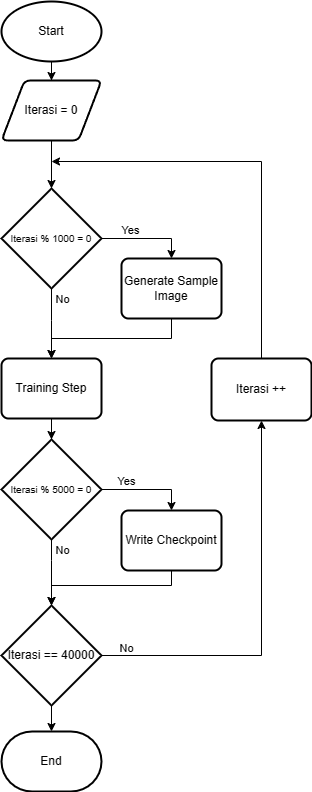
\includegraphics[scale=0.47]{gambar/Training_model.png}
  \caption{Flowchart Proses Training Model Keseluruhan}
  \label{fig:training}
\end{figure}

Untuk setiap 1 iterasi proses training, model akan menjalankan proses yang alurnya dapat dilihat pada gambar \ref{fig:arsitekturGAN}. 
Gambar Input akan dimasukkan ke Generator, dan akan menghasilkan Gambar sintesis. 
Discriminator akan memproses 2 pasangan input, yaitu pasangan gambar input dengan gambar asli, dan pasangan gambar input dengan gambar sintesis. 
Pada pasangan pertama, akan diperoleh output Discriminator dari gambar asli, dan pasangan kedua akan diperoleh output Discriminator dari gambar sintesis. 

Generator Loss akan memproses output Discriminator dari gambar sintesis, bersama dengan gambar hasil sintesis dan gambar asli. 
Hasil dari Total Generator Loss akan diterima oleh Generator Optimizer, dan akan diterapkan ke Generator di iterasi berikutnya. 
Discriminator Loss akan memproses output Discriminator dari gambar sintesis dan dari gambar asli. 
Hasil dari Total Discriminator Loss akan diterima oleh Discriminator Optimizer, dan akan diterapkan ke Discriminator di iterasi berikutnya.

\subsection{Evaluasi Model}
\label{subsec:evaluasi}

Setelah model mengalami proses training, model akan dites dengan menggunakan test data. 
Test data berupa 40 data dari dataset yang belum dilatih pada model. 
\emph{Checkpoint} yang disimpan terakhir akan dimuat, dan akan dicoba untuk mensintesis gambar menggunakan test data tersebut. 

Proses evaluasi dilakukan dengan evaluasi matriks kemudian dilanjut dengan evaluasi visual. 
Evaluasi matriks adalah metode objektif yang menggunakan berbagai metrik dan parameter numerik untuk mengukur sejauh mana dua gambar cocok atau berbeda. 
Metode evaluasi matriks yang digunakan pada penelitian ini adalah metode \emph{Root Mean Square} (RMS), \emph{Mean Square Error} (MSE) dan \emph{Structural Similarity Index} (SSIM). 
RMS dan MSE umumnya digunakan untuk mengukur kesalahan atau perbedaan antara dua gambar atau sinyal, dengan nilai yang lebih rendah menunjukkan kesamaan yang lebih besar. 
Sedangkan SSIM memberikan ukuran yang lebih holistik tentang kesamaan struktural antara dua gambar.

Setelah melakukan evaluasi matriks, dilakukan evaluasi visual. 
Evaluasi visual dilakukan dengan melibatkan penilaian subjektif oleh manusia terhadap kualitas dan kemiripan dua gambar. 
Dalam membantu proses evaluasi visual, digunakan fungsi \emph{image differencing}. 
Fungsi \emph{image differencing} melibatkan pengurangan piksel-piksel dari gambar asli dengan gambar sintesis. 
Hasil pengurangan dapat mengungkapkan informasi penting tentang perubahan struktur, pergeseran objek, atau perubahan lainnya dalam gambar.

\section{Bahan dan Peralatan yang Digunakan}
\label{sec:bahanPeralatan}

\subsection{GprMax}
\label{subsec:GprMax}

GprMax merupakan perangkat lunak open source yang mensimulasikan perambatan gelombang elektromagnetik. 
GprMax menggunakan metode Finite Difference Time-Domain (FDTD) dalam pemodelan numerik sinyal GPR. 
Kode pada gprMax aslinya berbasis C, dan sekarang sudah sepenuhnya ditulis ulang menggunakan kombinasi bahasa Python dan Cython. 
GprMax menggunakan file berbasis teks di mana setiap parameter simulasi ditentukan oleh pengguna. 
Parameter tersebut antara lain ukuran model, diskritasi, waktu simulasi, bentuk geometri, material, dan eksitasi.

\subsection{Jupyter Notebook}
\label{subsec:jupyter}

Jupyter Notebook merupakan aplikasi web untuk membuat dan membagikan dokumen. 
Dokumen biasa berisi kode, persamaan matematika, visualisasi gambar, maupun teks. 
Jupyter Notebook disajikan dalam bentuk kernel IPython, sehingga memungkinkan pengguna untuk menulis program dengan bahasa Python. 
Pada gprMax, Jupyter Notebook merupakan salah satu tools yang dapat digunakan dalam memplot sinyal GPR.

\subsection{Laptop}
\label{subsec:laptop}

Pada penelitian ini, alat utama yang akan digunakan adalah Laptop Asus TUF Gaming A15 FA506QM dengan Processor AMD Ryzen 7 @ 3.20Ghz, 
Ram 32 GB, 1 TB SSD, NVIDIA Geforce RTX 3060 dan AMD Radeon ™ Graphics Card, serta Sistem Operasi Windows.
